% The following list briefly describes the main observations of the results, before giving a more detailed evaluation in the following sections.
% \begin{enumerate}
%     \item Representing about half of the stalls, \textit{Sync \& control} stalls dominate in the baseline version of \Gls{vortex}. Removing unnecessary frontend stalls, allow the final version to heavily reduce the occurrence of \textit{sync \& control} stalls.
%     \item Compute bound benchmarks see great reductions in \acrshort{cpi} when increasing the throughput of the frontend and implementing ready scheduling, eliminating missed schedules.
%     \item The reduction in \textit{sync \& control} stalls is in most cases revealing more memory stalls.
%     \item Some benchmarks see a significant increase in idle cycles after implementing the changes.
%     \item For some benchmarks \textit{sync \& control} stalls are replaced by \textit{empty ibuffer} stalls.
%     \item For most benchmarks the scheduling algorithm has little to no effect on the performance.

% \end{enumerate}

% However most of the remaining stalls are data dependency stalls and missed schedules. The data stalls are mostly \textit{compute data} stalls, which are low latency, meaning the instructions will be ready in few cycles. By scheduling the ready instructions, and removing missed schedules, the low latency data stalls can be hidden until their operands become available.

% Increasing the throughput of the frontend makes more instructions available in the instruction buffer. This will also increase the number of available warps for the instruction scheduler. This together with a ready scheduler, allows \Gls{vortex} to issue additional instructions as long as they are ready. In the case of \textit{psort}, the number of stalls is halved, resulting in a decrease in \acrshort{cpi} by $20\%$. The number of frontend stalls is low for \textit{psort}. Thus it is seeing limited improvements from the frontend changes. However most of the remaining stalls are data dependency stalls and missed schedules. The data stalls are mostly \textit{compute data} stalls, which are low latency, meaning the instructions will be ready in few cycles. By scheduling the ready instructions, and removing missed schedules, the low latency data stalls can be hidden until their operands become available.


% For \textit{lavaMD} (Figure \ref{fig:instr_dist_lavaMD}), the distribution is skewed. In the baseline version, the highest throughput \acrshort{sm} executed $5.5\times$ more instructions than the \acrshort{sm} with lowest throughput. The distribution gets even worse when implementing the changes, making some of the \acrshortpl{sm} execute close to $0\%$ of the instructions. As LavaMD has close to none \textit{idle} stalls, the discrepancy is clearly not due to inactive \acrshortpl{sm}. Rather it is probable that the \acrshort{noc} is unable to distribute the bandwidth evenly among the \acrshortpl{sm}, resulting in different memory stalls for different \acrshortpl{sm}. The instruction distribution of \textit{backprop} is however even, thus the \acrshort{noc} cannot be at fault for \textit{backprop's} increase in \textit{memory structural} stalls. Unlike lavaMD, backprop use a lot of memory barriers. When a barrier is issued to the \acrshort{lsu}, all in-flight memory instructions have to complete before the \acrshort{lsu} become ready. For the benchmarks with \textit{memory structural} stalls and low bandwidth requirement, barriers are likely to be the cause.  
% This may indicate that the \acrshort{noc} is treating \acrshortpl{sm} unfairly, giving some of the \acrshortpl{sm} significantly less bandwidth than others. The throttled \acrshortpl{sm} would in that case stall due to \textit{memory structural stalls}, while the other \acrshortpl{sm} would be more dominated by \textit{memory data} stalls.

% \textcolor{red}{We observed a set of potential issues with Vortex. The issue scheduler does not have enough information to schedule ready warps. The front-end is unable to provide enough instructions to the issue stage, resulting in less scheduling opportunities.}

% \begin{figure}
%     \centering
%     \includegraphics[width=0.5\textwidth]{example-image-b}
%     \caption{CPI stacks for only baseline}
%     \label{fig:cpi_baseline}
% \end{figure}


% \textcolor{red}{Additionally, we observe that the front-end is unable to bring enough instructions to the issue stage. see \ref{fig:cpi_baseline}}

% \begin{figure}
%     \centering
%     \includegraphics{}
%     \caption{Caption}
%     \label{fig:enter-label}
% \end{figure}

%\textcolor{red}{The baseline issue scheduler checked if the scheduled instruction could be issued after scheduling. This resulted in cycles where warps where not scheduled even tough there ready warps were available}

%\textcolor{red}{This was solved by redesigning the issue stage as shown in \ref{fig:new_issue_stage}}

%\textcolor{red}{For all warps, check if they can issue. Most of the logic is implemented in scoreboard and dispatch. Requires selector in dispatch and scoreboard for each warp to read registers regarding the ready state}

% \textcolor{red}{While Vortex allows for FPGA simulation, it has a main issue, memory bandwidth and latency scaled to the throughput of the GPU. While work is being done at CAL to solve this, I have to continue using software simulation. }

% TODO: Comment on the number of bits used to track gto age and handling of overflow
% TODO: Comment on the size of the ibuffer

% \section{Allocating Memory}

% \textcolor{red}{celenqueuecopybuffer}
% During the porting of the \Gls{rodinia} benchmarks, I observed that\texttt{clEnqueueNDKernels} and \texttt{clCreateBuffer} either aborted or resulted in segmentation faults. Looking into the cause of this crash, I found that \texttt{clEnqueueNDKernels} caused a segmentation fault when the kernel contained local parameters. It seems like the driver is unable to dynamically allocate local memory for the local work groups. To solve this, we hardcoded the local buffers in the kernel scope before compiling the kernels. This introduces a new challenge of selecting the correct buffer size, corresponding to the problem size. Luckily we can just use the size given to \texttt{clSetKernelArg} when setting the local parameters. Still it requires to recompile the kernels when changing input size.

% To improve the insight into Vortex' performance, I expand upon my previous method for generating \textit{cycle-stacks for Vortex}(\acrshort{csv}), giving greater insight into what is causing Vortex to stall. Lastly I broaden Vortex' lacking benchmark suite by implementing benchmarks from Rodinia, a commonly used set of \acrshort{gpu} benchmarks. 

% On average, the frontend improvements reduce the number of frontend stalls by $71\%$. For benchmarks such as \textit{sfilter}, over $99\%$ of the frontend stalls are removed, as all the control stalls are unnecessary and removed. 
% The frontend changes heavily reduce the number of stalls caused by \Gls{vortex}' mechanisms to handle control flow. Together with the new schedulers it allows the issue stage to utilize its functional units to a greater degree. The changes give an average reduction in \acrshort{cpi} of --\% over the baseline, with \textit{psort}, \textit{sgemm} and \textit{Needleman-Wunsch} seeing a 20\% reduction in \acrshort{cpi}. However, some benchmarks see a slight increase or no change to their \acrshort{cpi}. This is due to a lack of memory bandwidth and \acrshort{mlp}, which can be solved by increasing the number of warps per \acrshort{sm}, and use a memory system more suitable for \acrshortpl{gpu}. I observe little to effect of using \acrshort{gto} over \acrshort{lrr}, which is likely due to weaknesses in my implementation. 

%In this thesis, I implement \textit{no-stall-scheduling} and \textit{stall-prediction} allowing vortex to schedule consecutive warps without stalling the frontend, and improve its icache-stage to increase throughput of the fetch stage. Additionally I improve Vortex' schedulers to detect ready warps, removing unnecessary stalls. I also examine the impact of switching from a \textit{loose-round-robin}(\acrshort{lrr}) to a \textit{greedy-then-oldest}(\acrshort{gto}) scheduling algorithm.

% \acrshort{fpga}-akselerasjon fungerer som en middelvei mellom softwaresimulering og maskinvareprototyper, ved å kombinere raske simuleringer med muligheten til å gjøre endringer raskt. Vortex er en RISC-V-basert GPGPU som kan FPGA-akselereres, og kan dermed være en god kandidat for forskning innen \acrshort{gpu} arkitekturer. Tidligere undersøkelser har funnet potensielle flaskehalser i \Gls{vortex}’ frontend og skedulerere. Dette hindret \Gls{vortex} i å utnytte \acrshort{simd} og \acrshort{mlp}, noe som reduserte gjennomstrømningen og gjorde den latensbundet.

% I denne oppgaven implementerer jeg \textit{no-stall-scheduling} og \textit{stall-prediksjon} som gjør det mulig for \Gls{vortex} å skedulere påfølgende warps uten å blokkere dem i frontenden. I tillegg forbedres icache-stadiet ved å øke gjennomstrømmingen av instruksjoner fra instruksjons-cachen. Jeg forbedrer også
% \Gls{vortex}’ skeduler, slik at den kan identifisere warps som er klare, dette fjerner unødvendige ventesykler. Jeg undersøker også virkningen av å bytte fra en \textit{loose-round-robin} (LRR) til en \textit{greedy-then-oldest} (GTO) algoritme for skedulering.

% For å forbedre innsikten i Vortex’ ytelse, utvider jeg mine tidligere
% implementasjon for å generere \textit{cycle-stacks for Vortex} (CSV), for å gi innblikk i
% hva som får Vortex til å sakke ned. Til slutt utvider jeg Vortex' manglende benchmark-suite
% ved å implementere benchmarks fra Rodinia, et ofte brukt sett med GPU-benchmarks.

% Endringene i frontenden reduserer antallet ventesykler forårsaket av \Gls{vortex}'
% mekanismer for å håndtere kontrollflyt. Sammen med de nye skedulererene muliggjør det for
% issue-stadiet å utnytte de funksjonelle enhetene i større grad. Forandringene
% gir en gjennomsnittlig reduksjon i \acrshort{cpi} på –\% over utgangspunktet, hvor \textit{psort, sgemm} og
% \textit{Needleman-Wunsch} ser en reduksjon i \acrshort{cpi} på $20\%$. Noen benchmarks
% opplever en liten økning eller ingen endring i \acrshort{cpi}. Dette skyldes en mangel på minne
% båndbredde og minnenivå parallellitet, som kan løses ved å øke antall warps per
% \acrshort{sm}, og bruk et minnesystem som er mer egnet for GPUer. Jeg observerer få forskjeller i bruk av
% GTO over LRR, noe som sannsynligvis skyldes svakheter i implementasjonen min.

%  They implemented a 3D graphics rendering accelerator supporting the Vulkan API, a modern graphics rendering API compared to the commonly used older OpenGL API. They also introduce a \Gls{riscv} \acrshort{isa} for accelerating graphics rendering, as well as implementing a compiler-driven control-flow divergence transformation to handle rendering loops inside graphics kernels. While \Gls{vortex} provides hardware texture units, Skybox has a hardware rasterizer and \acrfull{rop}. This results in a GPU more suitable for graphics workloads than \Gls{vortex}, as the \Gls{vortex} GPGPU is mostly suited for compute workloads.

% \Acrfullpl{gpu} are accelerators designed for executing highly parallelizable workloads. They are able to achieve high throughput by exploiting \acrfull{simt}. GPUs have a number of \acrfullpl{sm}, each with a set of parallel execution lanes, which can execute a set of logically independent threads. These threads are all a part of the same program known as the kernel. The programming model of GPUs is \textit{data-parallel}, that is the program is divided into a set of threads, all executing the same program, but with different data. As illustrated in Figure \ref{fig:kernel_work_items}, the kernel is divided into threads which is grouped into blocks called \acrfullpl{tb}. These \acrshortpl{tb} are then allocated and executed on the \acrshortpl{sm} in the \acrshort{gpu}. The \acrshortpl{sm} can be allocated a number of \acrshortpl{tb} at the same time. During execution, each \acrshort{sm} can execute \textit{warps} from all of its allocated \acrshortpl{tb}. A \textit{warp} is the next instruction in a \acrshort{tb} and is the basic execution unit of the \acrshort{gpu}. The threads within a warp run in lock-step, this means that all the threads execute the same instruction. In the case of divergence between threads, the branching threads are disabled, while the non-branching threads continue execution until their paths rejoin.

% For benchmarks with multiple kernels, the start-up time of each kernel become a relevant if the benchmark is not exited by early part of the performance

% Software simulation is much slower than running on ASICs or FPGAs. To keep the simulation time reasonable, I implement fast-forwarding, warm-up and early termination. \textit{Early termination} is implemented such that when \Gls{vortex} has ran for a given number of cycles, it jumps to the exit routine and dumps all performance metrics. This allows us to run benchmarks with realistic working-sets, to obtain realistic performance metrics. It is not ideal to terminate early, as the full behaviour of the benchmarks might not be captured. Additionally will changes to the architecture change the number of instructions executed within the simulated cycles. This is still a common solution \cite{simpoint}, as there are not many other options. Due to the increased number of benchmarks it is still likely that the results will be representable of \Gls{vortex}' performance.  

% It would be ideal to terminate based on the number of instructions committed, such that benchmark behaviour would be independent of changes to performance. However, as each core terminate based on internal metrics, cores with idle warps, would commit less instructions, using a disproportionate number of cycles compared to a core full of active warps. Thus I decided to terminate early based on cycle count.

% \textit{Fast-forwarding} is done by not collecting performance metrics in the start of the simulation. When doing early termination, the start of the simulation (e.g starting warps) represents a larger proportion of the total run-time. Not including the start-up, is thus important to obtain performance metrics representing the majority of the runtime. \textit{Warm-up} is removing the cold-start bias occurring at the beginning of the benchmark. This is due to empty caches, branch buffers, pre-fetchers, etc. By extending the number of cycles fast-forwarded, the GPU can be warmed up to give a more stable performance when simulating less cycles.

% Initially the L1 and L2 cache hit-rates were collected for a subset of the benchmarks. These are plotted in \ref{fig:l1_cache_hitrate} and \ref{fig:l2_cache_hitrate} for L1 and L2 cache respectively. After 30000 cycles, the cache hit-rate is stabilizing for both the L1 and L2 cache. While the L1 hit-rate for backprop is fluctuating, this is probably due to its access pattern, as similar fluctuations show up. To give some extra margins, 50000 was selected as the number of cycles to fast-forward.

% For benchmarks with multiple kernels, the start-up time of each kernel become a relevant if the benchmark is not exited by early part of the performance...

% \textcolor{red}{Some of the benchmarks did not run on idun, probably due to compiler differences}

% The existing benchmarks included with \Gls{vortex} are quite simple. They all consist of one kernel which is ran once, while most of the \Gls{rodinia} benchmarks contain multiple kernels. In the current version of Vortex a reset signal is sent to the \acrshort{gpu} before executing a kernel. This resets the GPU, including the registers holding the performance metrics to a known initial state. Thus if a benchmark executes multiple kernels, only the performance metrics of the last kernel persists. 

% As the kernels can have different characteristics, it is ideal to collect performance data for the entire benchmark. To make this possible, we have to stop the performance data from resetting. To achieve this we implemented a \acrfull{plr} which, when high, prevents the performance registers from resetting. This register is a \acrfull{csr} which can be written to using CSR-instructions, and is not affected by reset.

% To initialize the performance metrics, we have to queue a program which clears the \acrshort{plr}. By doing this, the performance metrics can reset before executing the next kernel. All consecutive kernels can set this register high to prevent the parameters from resetting. This allows for collecting performance metrics for the entire benchmark for multi-kernel benchmarks.

% \texttt{Dumping performance metrics at the end of the kernel}

% \textcolor{red}{Benchmarks are too long to run in software simulation, introduce early exit and warp-up. How was this implemented in vortex}

% \textcolor{red}{When implementing early exit, a problem arose, some benchmarks had exit conditions based on the result of their kernel. When using early exit, the result data my be garbage and result in infinite loops. To resolve this each benchmark had to be inspected to find loops and branches with conditions based on the kernel results and add safeguards, such as max number of iterations}

% \section{Cactus}

% \textcolor{red}{This could possibly be related work:}

% \textcolor{red}{Cactus vs Rodina, problematic to implement too many kernels. Rodinia is nice, because it usually between 1 and 3 kernels, easier to capture the behaviour when using software simulation, as the benchmarks cannot run long enough to capture behaviour from all kernels}

% For all benchmarks, most of the stalls in the baseline related to the issue stage are data stalls, i.e. \textit{memory data} and \textit{compute data} stalls. As there are few structural stalls it indicates that the throughput of the functional units are not fully utilized, I.e. \Gls{vortex} is latency bound. If there were more warps or other independent instructions available, they could be issued. With the increased throughput of the frontend, more warps are become available in the instruction buffer. For \textit{hotspot, 3D, lavaMD, backprop, saxpy, vecadd} and \textit{gaussian}, \textit{memory structural} stalls are exposed. This shows that the improvements are able to utilize the throughput of the \acrshortpl{lsu}. The reason why no \textit{compute structural} stalls are exposed is that most compute units have a throughput of one warp per cycle. 

% \textcolor{red}{If one of the ibuffers is full, it may cause backpressure into decode and fetch. Even if the icache stage has ready instructions, they cannot be decoded and issued. This may result in a state where only one warp is available in the ibuffer, while decode and the icache stage is stalling because it is waiting for the correct ibuffer slot to be available. If this warp is stalled due to a long latency stall, no other warps can be issued to hide the stall}

% \textcolor{red}{Figure \ref{fig:backpressure} shows the number of cycles per instruction where a warp is blocked in decode because of full ibuffers. ** Describe Notable elements of the graph **}

% \textcolor{red}{To resolve this issue, a signal is sent from the ibuffer to the warp scheduler and (icache stage for selector) indicating for each ibuffer if it is full or not}

% \begin{figure}
%     \centering
%     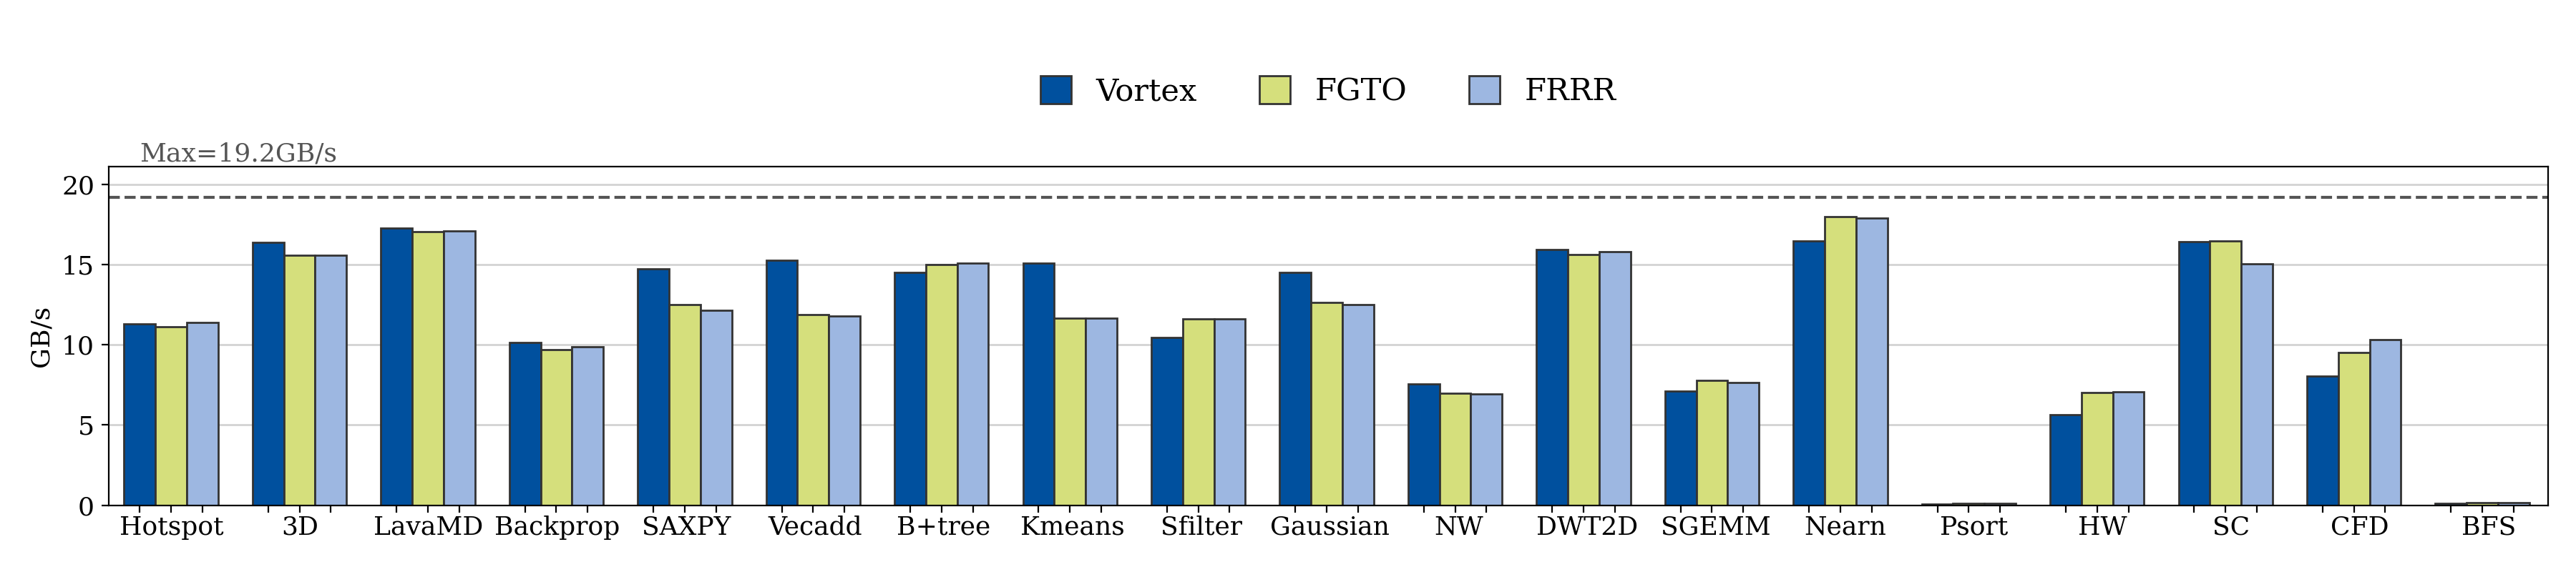
\includegraphics[width=\textwidth]{figures/backpressure/L2.png}
%     \caption{Backpressure, placeholder}
%     \label{fig:backpressure}
% \end{figure}

% \textcolor{red}{An alternative solution would be to implement a reset instruction, but the additional kernel would still be required. This solution less ideal, because the performance metrics would not be reset at the beginning of the benchmark, thus not include cycles of icache misses etc.}

% My solution to these issues is to create two additional kernels for collecting performance metrics, \textit{performance initializer} and \textit{performance dump}. First, the \textit{performance initializer} kernel sets the \texttt{perf-reset-lock} and \texttt{perf-lock} low, such that it resets upon starting the first kernel from the benchmark. Each kernel in the benchmark then set \texttt{reset-lock} high. This solves problem 4. At the end of the benchmark, the \textit{performance dump} kernel sets the \texttt{perf-lock} high before writing the data to memory, locking the performance data solves the first issue. Having a separate kernel for reading performance data, allows us to wait until the benchmark is completed before reading the data, thus solving problem 2 and 3.

% \textcolor{red}{Init kernel: ensure that the performance metrics are reset at the beginning of the benchmark. This is required as the reset lock register cannot be controlled by anything other than instructions}
% \textcolor{red}{Include in start.S that all kernels start by setting the reset lock, this is only required for the first kernel in the benchmark, but as it is implemented in start.S which is linked to all kernels, every kernel performs the action}
% \textcolor{red}{Dump kernel: ensure that the performance metrics are reset at the beginning of the benchmark}

% \Gls{vortex} allows for selecting between a set of different simulation environments, which are displayed in Figure~\ref{fig:simstack}. The available environments are the OPAE driver, VLSIM, RTLSIM and SIMX. The OPAE driver makes use of Intel's propretary AFU simulation environment (ASE). Both VLSIM and RTLSIM utilize Verilator to simulate the RTL design and use Ramulator~\cite{Ramulator}, an extensible DRAM simulator providing cycle-accurate performance models, to simulate memory in software. VLSIM additionally simulates the AFU in software. The SIMX driver implements a cycle-level simulator for \Gls{vortex}. All of these drivers share a common API when executing programs. 

% In the following sections I will present the results of the changes described in Chapter \ref{chap:changes}. The following list of configurations were tested.

% \begin{itemize}
%     \item \textbf{Vortex} is the baseline version of \Gls{vortex} as presented at MICRO'21 \cite{vortex}.
%     \item \textbf{RI} implements the new issue stage using ready-round-robin scheduling.
%     \item \textbf{GTO} Use GTO in warp scheduler and instruction scheduler. Both BPR and no-stall-scheduling (NSS) is enabled.
%     \item \textbf{RR} Use round-robin and ready-round-robin in the warp scheduler and instruction scheduler respectively. Both BPR and no-stall-scheduling (NSS) is enabled.    
% \end{itemize}

% \textcolor{red}{For most of the benchmarks, memory instructions become the largest source of stalls. Note that for all benchmarks except lavaMD, \textit{memory data stalls} are more prevalent than \textit{memory structural stalls}. The \acrshort{lsu} is thus capable of handling more loads. This may indicate that the GPU is latency bound and not bandwidth bound. Increasing the number of warps in each core may introduce more \acrfull{mlp} and thus hide the latency stalls.}

% \textcolor{red}{Doubling the number of warps in each core will alter the number of work items per wave and can thus result in a different number of instructions required to complete the execution of the program. Additionally, the . To ensure that the results are comparable with the results using 4 warps there is no artificial increase in IPC due to sche}

% Some benchmarks see great performance improvements, while others reveal that \Gls{vortex} struggles to hide latencies. I also find that the current configuration is too small to gain performance from \acrshort{gto} over \acrshort{lrr} scheduling. This constitutes contribution \textbf{C3} corresponding with task \textbf{T3}.

% - Figure shows 
% - Baseline has a larger proportion of frontend stalls, as it is unable to schedule instructions to fill the increased width of the instruction buffer
% - The new frontend is able to throughput enough instructions
% - Increase in memory structural stalls and reduction in memory data stalls, this indicates that we are hitting the limit of the memory bandwidth.
% - More idle cycles due to more skew in bandwidth distribution because of more memory contention 

% -sgemm, psort and dwt see a great improvements
%  - psort bound by short latency compute data stalls,
%  - sgemm bound by memory latency, but its latency is lower than others
%  - dwt2d hard to say, something might be wrong 

% For \textit{NW}, the \acrshort{cpi} is drastically increased for \textit{FGTO} and \textit{FRRR}. As the L1 cache hit rate for \textit{NW} is low, removing the L2 cache will cause a large number of requests to be sent to the main memory. Because of this, there might be a substantial amount of queuing in the memory system, especially when using \textit{FGTO} and \textit{FRRR}. While the latency of reading main memory is high, the increased throughput is thus increasing it even further. This   .in the memory system, which further increases it. As memory latency is already the bottleneck for \textit{NW}, increasing frontend throughput and issue bandwidth hurts performance when using only L1 caches.

% By only incrementing the age upon a schedule, the age registers does not require many bits to track the age of the warps. In my case, I found that  than if the age was incremented every cycle.

% Accelerators are a common method to increase  \acrfull{hpc} to increase computing power. Accelerators have compute units specialized for a single domain. \acrshortpl{gpu} are by far the most common type of accelerator, exploiting data level parallelism to achieve high throughput for highly parallelizable workloads. \acrshortpl{gpu} are used for graphics operations, but also for other more compute focused workloads. Due to the prevalence of \acrshortpl{gpu}, \acrshort{gpu} research is becoming more essential.

% \textcolor{red}{This is a part of enabling GPU research at in CAL at NTNU.}

% \textcolor{red}{Describe why FPGA simulation is great and why this is a motivation for using vortex. A common method for evaluating computer architecture is software simulation. This is troublesome for larger systems as it is slow}

% \textcolor{red}{This work is also about getting to know Vortex and its architecture. Improving the Vortex environment with benchmarks and tools (\acrshort{csv}) which can be used on FPGAs}